% !TeX spellcheck = hr_HR
\documentclass[times, utf8, diplomski]{fer}
\usepackage{booktabs}
% razno
\usepackage{amsmath}
\usepackage{mathtools}
\usepackage{graphicx}
\usepackage{float}
\usepackage{amssymb}
\usepackage{geometry}
\geometry{margin=2cm}
\usepackage{seqsplit}
\usepackage{times}
\usepackage[T1]{fontenc}
\usepackage[ddmmyyyy]{datetime}
\usepackage{verbatim}
\usepackage[croatian]{babel}
\usepackage{todonotes}

%matlab - importanje
\usepackage{listings}
\usepackage{color} %red, green, blue, yellow, cyan, magenta, black, white
\definecolor{mygreen}{RGB}{28,172,0} % color values Red, Green, Blue
\definecolor{mylilas}{RGB}{170,55,241}


%counter reset - counteri za equatione figure itd.
\usepackage{chngcntr}
\counterwithout*{equation}{chapter}
%\counterwithin*{equation}{subsection}
% \counterwithin*{figure}{section}
\counterwithin*{figure}{chapter}
% \counterwithout*{figure}{section}
% \counterwithin*{figure}{subsection}

%pretty formating - formatiranje raznih 
\renewcommand{\thechapter}{\arabic{chapter}}
\renewcommand{\thesection}{\arabic{chapter}.\arabic{section}}
\renewcommand{\theequation}{\arabic{chapter}-\arabic{equation}}
\renewcommand{\thefigure}{\arabic{chapter}-\arabic{figure}}

%centering figure captions - workaround!
{\makeatletter\long\gdef\@gobble#1{}}
\usepackage[justification=centering]{caption}

%calligraphy packages
\usepackage{calrsfs}
\DeclareMathAlphabet{\pazocal}{OMS}{zplm}{m}{n}
\newcommand{\Ca}{\pazocal{C}}
\newcommand{\Oa}{\pazocal{O}}
\newcommand{\Va}{\pazocal{V}}
\newcommand{\Ua}{\pazocal{U}}
\newcommand{\Aa}{\pazocal{A}}


\usepackage{amsmath}

\begin{document}
	% za importanje matlab kodova
	\lstset{language=Matlab,%
		%basicstyle=\color{red},
		breaklines=true,%
		morekeywords={matlab2tikz},
		keywordstyle=\color{blue},%
		morekeywords=[2]{1}, keywordstyle=[2]{\color{black}},
		identifierstyle=\color{black},%
		stringstyle=\color{mylilas},
		commentstyle=\color{mygreen},%
		showstringspaces=false,%without this there will be a symbol in the places where there is a space
		%		numbers=left,%
		%		numberstyle={\tiny \color{black}},% size of the numbers
		%		numbersep=9pt, % this defines how far the numbers are from the text
		emph=[1]{for,end,break},emphstyle=[1]\color{red}, %some words to emphasise
		%emph=[2]{word1,word2}, emphstyle=[2]{style},    
	}
	
% TODO: Navedite broj rada.
\thesisnumber{1731}

% TODO: Navedite naslov rada.
\title{Geometrijsko upravljanje multirotorskom letjelicom s benzinskim motorima}

% TODO: Navedite vaše ime i prezime.
\author{Lovro Marković}

\maketitle

% Ispis stranice s napomenom o umetanju izvornika rada. Uklonite naredbu \izvornik ako želite izbaciti tu stranicu.
\izvornik

% Dodavanje zahvale ili prazne stranice. Ako ne želite dodati zahvalu, naredbu ostavite radi prazne stranice.
\zahvala{}

\tableofcontents

\chapter{Uvod}

\paragraph{}
Cilj ovoga rada je razviti i implementirati nelinearno geometrijsko upravljanje za multirotorsku letjelicu s benzinskim motorima. U radu će najprije biti postavljeni temelji za razumijevanje geometrijskog načina upravljanjima sustavima. Zatim će biti predstavljen sustav multirotorske letjelice te način implementacije nelinearnog geometrijskog upravljanja za takav konkretan sustav. Naposlijetku bit će prikazani i komentirani dobiveni rezultati u Gazebo simulatoru. \\

\paragraph{}
TODO

\newpage 
\clearpage

\chapter{Diferencijalna geometrija}

\section{Uvod}
	\paragraph{} Upravljanje mehaničkim sustavima u nastavku ćemo provoditi geometrijskih metodama, odnosno metodama diferencijalne geometrije. Osnovna konstrukcija u diferencijalnoj geometriji je manifold. Ugrubo to je skup koji lokalno izgleda kao otvoreni podskup Euklidskog prostora. Na taj način manifold se može preciznije analizirati koristeći poznate konstrukcije iz analize Euklidskih prostora. \\ 
	Jedna bitna razlika između manifolda i Euklidskih prostora jest koordinatna invarijantnost. Postoji više načina pomoću kojih u manifoldu možemo naći lokalnu sličnost sa Euklidskim prostorom, ali je ključno da su te metode neovisne o proizvoljnim izborima kao što su pristranost određenim koordinatnim sustavim i slično. To ne znači da se ne potiče korištenje koordinatnih sustava već da same metode i koncepti koji su korišteni budu koordinatno invarijantni, ali prikazani u željenim koordinatama. \\
	U nastaku bit će definirana lokalna sličnost manifolda Euklidskom prostoru.

\section{Topološki prostor}
	
	\paragraph{}Neka je $S$ skup elemenata i $2^S$ je skup svih podskupova od $S$. Topološki prostor je par $(S, \Oa)$ gdje je $\Oa\subset2^S$ kolekcija svih podskupova, tj. otvoreni skup koji zadovoljava:
	\begin{enumerate}
		\item $\emptyset \in \Oa$ i $S \in \Oa$ 
		
		\item Ako je A proizvoljni skup cijelih brojeva i vrijedi da je $\{ \Oa_{a} \}_{a\in A}\subset \Oa$ proizvoljna kolekcija otvorenih skupova tada vrijedi $\bigcup_{a\in A}\Oa_a\in \Oa$, drugim riječima vrijedi da je $\Oa$ prebrojiv.
		
		\item Ako $\Oa_1, \Oa_2 \in \Oa$ tada $\Oa_1 \cap \Oa_2 \in \Oa$
	\end{enumerate}
	\paragraph{}Dakle, ako kažemo da je S topološki prostor, te vrijede prethodni uvjeti tada se pretpostavlja neka topologija $\Oa$ nad prostorom $S$.

\newpage
\clearpage

\section{Mape}

	\paragraph{}Neka su $(S, \Oa_s)$ i $(T, \Oa_t)$ topološki prostori i neka je $f:S \rightarrow T$ mapa, tada vrijedi:
	
	\begin{enumerate}
		
		\item Mapa je kontinuirana u $x_0$ za $x_0 \in S$ ako za svako susjedstvo $\Va$ od $f(x_0)$ postoji susjedstvo $\Ua$ of $x_0$ za koje vrijedi $f(\Ua)\subset\Va$ 
		
		\item Ako je mapa f kontinuirana za $\forall x \in S$ tada je mapa kontinuirana.
		
		\item Ako je f bijekcija, kontinuirana i ima inverz koji je također kontinuiran tada je mapa f homeomorfizam.
`	
	\end{enumerate}
	
	
\section{Diferencijalne mape višeg reda}

	\paragraph{} Neka je $\Ua$ otvoreni podskup $\mathbb{R}^n$ i neka je mapa $f: \Ua \rightarrow \mathbb{R}^m$ tada:
	\begin{enumerate}
		
		\item Ako postoji r-ta kontinuirana derivacija mape f tada je f r-puta diferencijabilna tj. klase $\boldsymbol{C}^r$ (kontinuirane mape su klase $\boldsymbol{C}^0$) .
		
		\item Ako je f klase $\boldsymbol{C}^r$ $\forall r \in \mathbb{N}$ tada je beskonačno diferencijabilna ili klase $\boldsymbol{C}^\infty$. Također se može reći da je mapa f glatka ako je klase $\boldsymbol{C}^\infty$.
		
		\item Mapa f je $\boldsymbol{C}^r$-difeomorfizam ako vrijedi da je bijekcija otvorenih skupova $f:\Ua \subset \mathbb{R}^n \rightarrow \Va \subset \mathbb{R}^m$, ako je klase $\boldsymbol{C}^r$ te ako je inverz mape f isto klase $\boldsymbol{C}^r$.
	
	\end{enumerate}
	
\section{Karte, atlasi i diferencijalne strukture}
	\paragraph{} Neka je $S$ skup. Karta od $S$ je par $(\Ua, \phi)$ sa svojstvima:
	\begin{enumerate}
		\item $\Ua$ je podskup od $S$
		\item $\phi: \Ua \rightarrow \mathbb{R}^n$ je injekcija pri kojoj je $\phi(\Ua)$ otvoreni podskup od $\mathbb{R}^n$
		
		$\boldsymbol{C}^r$ - atlas od $S$ je skup $\Aa = \{ (\Ua_a, \phi_a) \}_{a\in A}$ karata sa svojstvom da je $S = \cup_{a\in A}\Ua_a$ te kadgod je zadovoljeno $\Ua_a \cap \Ua_b \neq \emptyset$ tada dalje vrijedi:
		
		\item $\phi_a(\Ua_a \cap \Ua_b)$ i $\phi_b(\Ua_a\cap \Ua_b)$ su otvoreni podskupovi od $\mathbb{R}^n$
		\item Tranzijentna mapa $\phi_{ab} \triangleq \phi_b \circ \phi_a^{-1}$ je $\boldsymbol{C}^r$ - difeomorfizam od $\phi_a(\Ua_a \cap \Ua_b)$ prema $\phi_b(\Ua_a\cap \Ua_b)$.
	\end{enumerate}
	
	Ekvivalenciju među više atlasa možemo uspostaviti na slijedeći način. Neka su dana dva $\boldsymbol{C}^r$-atlasa $\Aa_1$ i $\Aa_2$. Oni će biti ekvivalentni ako je vrijedi da $\Aa_1 \cup \Aa_2$ je isto $\boldsymbol{C}^r$-atlas. Nadalje se može definirati $\boldsymbol{C}^r$-diferencijabilna struktura na skupu S kao klasa ekvivalencija atlasa sa prethodno definiranom relacijom ekvivalencije dvaju atlasa. \\
	Naposlijetku definiramo $\boldsymbol{C}^r$-diferencijalni manifold ili samo $\boldsymbol{C}^r$-manifold M kao skup S sa prethodno definiranom $\boldsymbol{C}^r$-diferencijalnom strukturom. Dakle manifold je skup S sa kolekcijom atlasa koji sadrže mape $\phi$ pojedinih područja $\Ua$ skupa S prema $\mathbb{R}^n$. \\
	Na isti način može se definirati i glatki manifold, odnosno $\boldsymbol{C}^\infty$-manifold. Takav manifold sadrži glatku diferencijalnu strukturu što podrazumijeva glatke mape preslikavanja u Euklidski prostor. U nastavku razmatrat će se upravo takve vrste manifolda.
	
	\begin{figure}[h]
		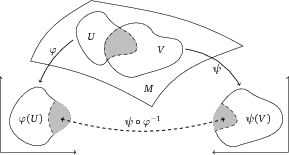
\includegraphics[width=\textwidth]{fig_overlap_charts.png}
		\caption{Grafički prikaz manifolda M te transportnih funkcija $\varphi$ i $\psi$ od manifolda $M$ prema $\mathbb{R}^2$ te prikaz kompozicije transportnih mapa kao vezu između slika preklopnih dijelova $\Ua$ i $\Va$ u Euklidskom prostoru.}
	\end{figure}

\section{Tangencijalni prostor na manifoldu}

	Neka je M manifold. Tada se može konstruirati vektorski prostor nad $\mathbb{R}$ na slijedeći način: $(\boldsymbol{C}^\infty(M), +, \cdot)$, gdje je $\boldsymbol{C}^\infty(M) = \{ f: M \rightarrow \mathbb{R} \ | f \,je\, glatka\}$. Dakle, definiran je vektorski prostor kao skup svih glatkih mapa $f$ sa pridruženim operatorima zbrajanja i množenja. 
	
	\paragraph{Krivulja na manifoldu:} Neka je definirana krivulja na manifoldu kao glatka mapa $\gamma:\mathbb{R} \rightarrow M$, gdje je $\mathbb{R}$ promatran kao 1-dimenzionalni manifold.
	
	\paragraph{Operator usmjerene derivacije:} Neka je $\gamma: \mathbb{R} \rightarrow M$ glatka krivulja kroz točku $p\in M$ te bez gubljenja općenitosti može se uzima se da vrijedi $\gamma(0) = p$. Tada se može definirati operator usmjerene derivacije duž krivulje $\gamma$ u točki $p$ kao mapu na slijedeći način: \\
	\begin{gather}
		X_{\gamma, p} : \boldsymbol{C}^\infty(M) \rightarrow R \\
		f \mapsto (f \circ \gamma)'(0)
	\end{gather}
	Bitno je primijetiti kako je kompozicija $(f \circ \gamma)$ mapiranje unutar realnog prostora tako da se toj funkciji na uobičajan način može pronaći i evaluirati derivacija.
	Intuitivno gledano $X_{\gamma, p}$ je brzina krivulje $\gamma$ u točki $p$.
	
	\paragraph{Tangencijalni prostor:} Neka je M manifold koji sadrži točku $p$. Tada je tangencijalni prostor vektorski prostor nad $\mathbb{R}$ sa skupom operatora usmjerene derivacije tako da vrijedi: \\
	$T_p M := \{ X_{\gamma, p} \, | \, \gamma \, je \, glatka \, krivulja \, kroz \, p\}$ te sa nadodanim operatorima zbrajanja i skalarnog množenja.
	
	\begin{figure}[h!]
		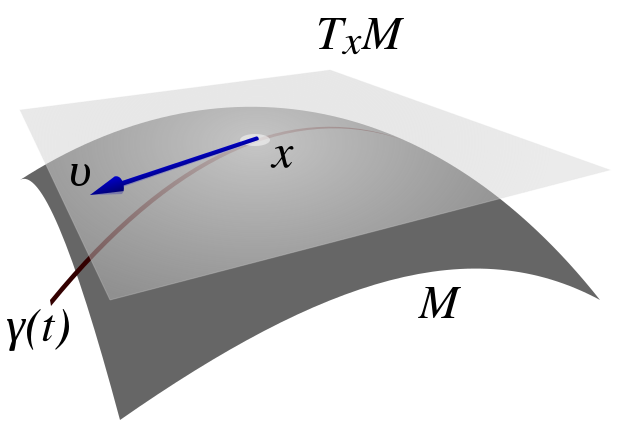
\includegraphics[width=\textwidth]{txm.png}
		\caption{Na slici je prikazan manifold M. Parametrirana krivulja $\gamma(t)$ koja prolazi točkom $x$. Tangencijalni prostor manifolda M u točki x $T_x M$ te vektor usmjerene derivacije $v$ krivulje $\gamma (t)$ u točki $x$. }
	\end{figure}
	
\chapter{Lijeve grupe i Lijeva algebra}

\section{Uvod}

	\paragraph{}Lijeva teorija je od velike važnosti i u fizici i u diferencijalnoj geometriji. U ovom dijelu bit će predstavljen koncept Lijeve grupe te pripadajuće Lijeve algebre. Fokus će biti usmjeren prema Specijalnim Euklidskim grupama SE(3) budući da su one predmet zanimljive u kontekstu ovog rada.
	
\section{Lijeve grupe}

	\paragraph{} Lijeva grupa je grupa $(G, \bullet)$ gdje je G glatki manifold klase $\boldsymbol{C}^\infty$, a $\bullet$ pripadajući operator nad G. Svojstva operatora $\bullet$ su slijedeća: 
	\begin{enumerate}
		\item Asocijativnost: $\forall a, b, c \in G :  a\bullet(b\bullet c) = (a\bullet b) \bullet c$
		\item Neutralni element: $\exists e \in G : \forall g \in G : g \bullet e = e \bullet g = g$
		\item Inverz: $\forall g \in G : \exists g^{-1} \in G : g \bullet g^{-1} = g^{-1} \bullet g = e$
	\end{enumerate}
	Ako vrijedi i svojstvo komutativnosti: $a \bullet b = b \bullet a, \forall a, b \in G$ tada je grupa abelijanska. Dana je toplogija nad G preko slijedećih mapa:
	
	\begin{gather}
		\mu: G \times G \rightarrow G \\
		(g_1, g_2) \mapsto g_1 \bullet g_2 \\ g_1, g_2 \in G
	\end{gather}
	
	i: 
	\begin{gather}
		i: G \rightarrow G \\
		g \mapsto g^{-1} \\
		g \in G
	\end{gather}
	
	Mape $g$ i $i$ su glatke mape. Dakle Lijeve grupe su topološke grupe, čiji se elementi unutar toploškim prostorom, odnosno dio manifolda, a operacija nad grupom $\bullet$ je kontinuirana, kao i njen inverz.

	\newpage
	\clearpage
	
\section{Specijalna euklidska grupa - SE(3)}

	\paragraph{}U ovom dijelu bit će definirano nekoliko različitih Lijevih grupa s konačnim ciljem definiranja specijalne ortogonalne grupe SO(3) te njenog proširenja na specijalnu Euklidsku grupu SE(3). 	
	
	\paragraph{N-dimenzijska translacijska grupa:} Mapa $\varphi$ je kruta mapa ako vrijedi 
	$\forall v, w \in \mathbb{R}^n, \, d(\varphi(v), \, \varphi(w)) = d(v, w)$. Drugim riječima mapa je kruta ako su nakon mapiranja duljine očuvane. \\
	Neka je skup $G$ sačinjena od svih krutih mapa tako da vrijedi $G = \{ \varphi: \mathbb{R}^n \rightarrow \mathbb{R}^n \, | \, \varphi\, je\, kruta\, mapa\} := T(n)$. Ako se skupu $T(n)$ pridruži operator kompozicije tada se dobiva translacijska Lijeva grupa $(T(n), \circ)$.
	
	\paragraph{Opća linearna grupa (\textit{"General linear group"}):} Neka je skup G sačinjen od matrica, tj. mapa $\varphi$ tako da vrijedi $G = \{ \varphi: \mathbb{R}^n \rightarrow \mathbb{R}^n \,|\, det \, \varphi \neq 0 \}:=GL(n, \mathbb{R}^n)$. Ako bi tome skupu pridodali operator kompozicije $\circ$ tada možemo definirati Lijevu grupu $(GL(n, \mathbb{R}^n), \circ)$. To je dakle grupa svih invertibilnih matrica koje svoje karakteristike glatkog manifolda naslijeđuju činjenicom da su takve matrice otvoreni podskup grupe svih nxn matrica $\mathbb{R}^{n^2}$ koje čine glatki manifold.
	\todo[inline]{Reci da je Rn2 stvarno glatki manifold (u appendixu?)}
	
	\paragraph{(Specijalna) Ortogonalna grupa:} Neka je skup G sačinjen od matrica $Q$ tako da vrijedi \\ 
	$G = \{ Q \in GL(n, \mathbb{R}^n) \,|\, det \, Q = \pm 1\} := O(n)$. Budući da su matrice elementi skupa $GL(n, \mathbb{R}^n)$ njima se može pridodijeliti i naslijeđeni operator $\circ$. Takva Lijeva grupa $(O(n),\circ)$ zove se ortogonalna grupa. \\
	Specijalna ortogonalna grupa $SO(n)$ je podgrupa ortogonalnoj grupi, uz uvjet da matrice moraju imati determinante jednake 1. Ta grupe se ujedno naziva i rotacijska grupa jer sadrži sve rotacijske matrice. \\
	Obje grupe lančano naslijeđuju karakteristike glatkog manifolda od opće linearne grupe.
	
	\paragraph{(Specijalna) Euklidska grupa:} Euklidska grupa kao podgrupe sadrži translacijsku Lijevu grupu $T(n)$ i ortogonalnu grupu $O(n)$. Svaki element u $E(n)$ sastoji se od translacije koju slijedi ortogonalna transformacija. \\
	Specijalna Euklidska grupa kao podskup umjesto ortogonalne grupe sadrži specijalnu ortogonalnu grupu. U tom slučaju svaki član te grupe sadrži translaciju koju slijedi rotacija. Elementi te grupe su (n+1)x(n+1) matrice slijedećeg oblika: \\
	
	\begin{equation}
		\left \{
		\begin{bmatrix}
		R_{3 \times 3} & v_{3 \times 1} \\
		0 & 1
		\end{bmatrix}
		\, \Biggr\rvert \, R \in SO(3) \, , \, v \in \mathbb{R}^n
		\right \} \in SE(3)
	\end{equation}	
	
\newpage
\clearpage

\section{Lijeva algebra}

	\paragraph{Algebra:} Algebra nad poljem K je skup od četiri elemenata $(A, +, \cdot, \bullet)$, gdje je $(A, +, \cdot)$ vektorski prostor nad poljem K, a $\bullet$ je produkt nad A, tj. bilinearno mapiranje: $\bullet : A \times A \rightarrow A$. \\
	Algebra $(A, +, \cdot, \bullet)$ može biti:
	\begin{enumerate}
		\item Asocijativna ako vrijedi $\forall v, w, z \in A : v \bullet (w \bullet z) = (v \bullet w) \bullet z$
		
		\item Unitalna ako vrijedi $\exists e \in A : \forall v \in A : e \bullet v = v \bullet e = v$
		
		\item Komutativna ili abelijanska ako vrijedi $\forall v, w \in A : v \bullet w = w \bullet v$
	\end{enumerate}
	
	\paragraph{Lijeva algebra:} Lijeva algebra je algebra čiji operator je Lijeva zagrada $[-,-]$ (tipično zvana komutator) za koju vrijede svojstva: 
	
	\begin{enumerate}
		
		\item Antisimetričnost: $\forall v \in A: [v, v] = 0$
		
		\item Jakobijev identitet: $\forall v, w, z \in A : [v,[w, z]] + [w,[z,v]] + [z,[v,w]] = 0$
		
	\end{enumerate} 
	
	Iz uvjeta o antisimetričnosti odmah vrijedi $[v,w]=-[w,v]$. Kod asocijativnih algebri komutator se definira kao $[v,w]:=v \bullet w - w \bullet v$.
	
	\paragraph{Lijeva algebra Lijeve grupe:} Svaka Lijeva grupa ima svoju pripadajuću Lijevu algebru. Lijeva algebra $g$ od Lijeve grupe $G$ je tangencijalni prostor oko točke identiteta $T_e G$.
	
	\paragraph{Eksponencijalna mapa:} Poveznica između Lijeve grupe i njene pripadajuće Lijeve algebre je eksponencijalna mapa. Ona je definirana na slijedeći način: $exp: T_eG \rightarrow	G$, tj. $exp: g \rightarrow G.$ \\ Postoji i logaritamska mapa koja služi za inverno mapiranje od Lijeve grupe prema pripadajućoj algebri.

\todo[inline]{Definirati diferencijalne mape između tangencijalnih prostora}
\section{Algebra specijalne ortogonalne grupe $so(3)$}

	Naposlijetku bit će potrebno definirati pripadajuću Lijevu algebru $so(3)$ nad Lijevom grupom SO(3). \\
	Lijeva algebra $so(3)$ je skup anti-simetričnih realnih matrica. Budući da je takav skup matrica proizašao iz tangencijalnog prostora rotacijske grupe SO(3) tada će te matrice zapravo predstavljati tenzore kutnih brzina oko neke konfiguracije $R$. \\
	Na primjer, ako je rotacija ua kut $\psi$ oko z-osi definirana kao:
	
	\begin{equation}
		R( \hat{e}_3, \psi ) = 
		\begin{bmatrix}
			cos(\psi)	&	-sin(\psi)	&	0 \\
			sin(\psi)	&	cos(\psi)	&	0 \\
			0			&	0			&	1 \\	
		\end{bmatrix} \in SO(3)
	\end{equation}
	
	\newpage
	\clearpage
	
	Ako se sada razvije matrica rotacije u Taylorov red prvog stupnja dobit će se matrica infinitiezimalne rotacije: \\
	\begin{equation}
		R( \hat{e}_3, \partial \psi ) = I + \partial \psi 
		\begin{bmatrix}
			0	&	-1	&	0 \\
			1	&	0	&	0 \\
			0	&	0 	&	0
		\end{bmatrix}
		= I + \partial \psi J_z
	\end{equation}
	\\
	\noindent Gdje je $J_z$ jedan od tri elementa koja definiraju bazu algebre $so(3)$. Ostali elementi baze su:
	
	\begin{equation}
		J_1 = 
		\begin{bmatrix}
		0	&	0	&	0 \\
		0	&	0	&	-1 \\
		0	&	1 	&	0
		\end{bmatrix} \\
		\, , \, J_2 = 
		\begin{bmatrix}
		0	&	0	&	1 \\
		0	&	0	&	0 \\
		-1	&	0 	&	0
		\end{bmatrix} 
	\end{equation}
	\\
	Još se nazivaju i generatori rotacije jer njihovim uzastopnim primjenjivanjem se postiže rotacija za željeni kut na slijedeći način:
	
	\begin{align}
		R( \hat{e}_3, \psi ) & = (I + \partial \psi J_z)^n \\
							 & = \lim_{n \rightarrow \infty} \left (I + J_z \frac{\psi}{n} \right )^n \\
							 & = e^{J_z \psi}
	\end{align}
	\\
	Iz gornje relacije se također vidi veza između matrice rotacije, elementa grupe SO(3), i generatora infinitezimalne rotacije, elementa algebre ($so(3)$), preko prethodno definirane eksponencijalne mape. \\
	Sada se može definirati opća rotacija oko vektora $\hat{n}$ za kut $\psi$ kao:
	
	\begin{equation}
		R( \hat{n}, \phi ) = e^{(J_1 n_1 + J_2 n_2 + J_3 n_3)\psi}
	\end{equation}
	\\
	Uzevši to u obzir, vektor kutne brzine $\vec{\omega} = [\omega_x, \omega_y, \omega_z]$, može se zapisati u obliku tenzora, tj. elementa algebre $so(3)$ kao: 
	
	\todo[inline]{Provjeriti u kodu matricu rotacije - bookmarkan wiki stranica}
	\begin{equation}
		\hat{\omega} = 
		\begin{bmatrix}
			0			&	-\omega_z	& 	\omega_y \\
			\omega_z	&	0			& 	-\omega_x \\
			-\omega_y	&	\omega_x	&	0
		\end{bmatrix} \, , \, \hat{\cdot}: \mathbb{R}^3 \rightarrow so(3)
	\end{equation}
	
	\noindent Gdje kapa-operator mapiranje iz Realnog 3-dimenzionalnog prostora prema Lijevoj algebri $so(3)$. Njemu inverzan operator je v-operator koja je definirana kao $\check{\cdot}:so(3) \rightarrow \mathbb{R}^3$.
	
\chapter{Matematički model letjelice}

\paragraph{}U ovom radu kao sustav upravljanja razmatra se multirotorska letjelica sa četiri rotora postavljena u plus konfiguraciju. Kao pomoć pri prikazivanju jednadžbi odabrana su dva koordinatna sustava: 
\begin{itemize}
	\item Globalni: $\{\vec{e}_1, \vec{e}_2, \vec{e}_3\}$
	\item Lokalni - tijelo letjelice: $\{\vec{b}_1, \vec{b}_2, \vec{b}_3\}$
\end{itemize}

\noindent Općenite jednadžbe gibanja takvog sustava su:
\begin{gather}
	\dot{x} = v \\
	m \dot{v} = mge_3 - fRe_3 \\
	\dot{R} = R\hat{\Omega} \\
	J\dot{\Omega} + \Omega \times J\Omega = M
\end{gather}

gdje je:
\begin{itemize}
	\item $x \in \mathbb{R}^3$ - trenutna pozicija letjelice
	
	\item $m \in \mathbb{R}$ - ukupna masa letjelice
	
	\item $f \in \mathbb{R}$ - ukupni potisak letjelice 
	
	\item $R \in SO(3)$ - matrica rotacije iz lokalnog u globalni koordinatni sustav
	
	\item $\Omega \in \mathbb{R}^3$ - kutna brzina letjelice u lokalnom koordinatnom sustavu
	
	\item $J \in \mathbb{R}^{3\times3}$ - matrica inercije letjelice s obzirom na lokalni koordinatni sustav
	
	\item $M \in \mathbb{R}^3$ - ukupni moment letjelice s obzirom na lokalni koordinatni sustav
\end{itemize}

\noindent Budući da se upravlja brzinom vrtnje rotora potrebna je poveznica sa ukupnom silom i ukupnim momentima. Ta dva pojma povezana su preko sile koju generira pojedini rotor $f_i$, a veza je slijedeća:

\begin{gather}
	f_i = \zeta_i b_f \Omega_{i}^2 \\
	M_i = b_m f_i
\end{gather}

gdje je:
\begin{itemize}
	\item $\zeta_i = 1,\, i = 2, 4$, $\zeta_i = -1,\, i=1,3$ zbog različitih smjerova vrtnje rotora
	\item $b_f$ - konstanta potiska motora
	\item $b_m$ - kontatnta momenta motora
\end{itemize}

\newpage
\clearpage

Radi lakše pretvorbe uvodi se matrični zapis na slijedeći način: 

\begin{equation}
	\begin{bmatrix}
		f \\
		M_1 \\
		M_2 \\
		M_3 
	\end{bmatrix} 
	=
	\begin{bmatrix}
		1	&	1	&	1	&	1 \\
		0	&	d	&	0	&	-d \\
		-d 	&	0	&	d	&	0 \\
		b_m &	-b_m	& 	b_m	& -b_m
	\end{bmatrix}
	\cdot
	\begin{bmatrix}
		f_1 \\
		f_2 \\
		f_3 \\
		f_4
	\end{bmatrix}
\end{equation}

\begin{figure}[h!]
	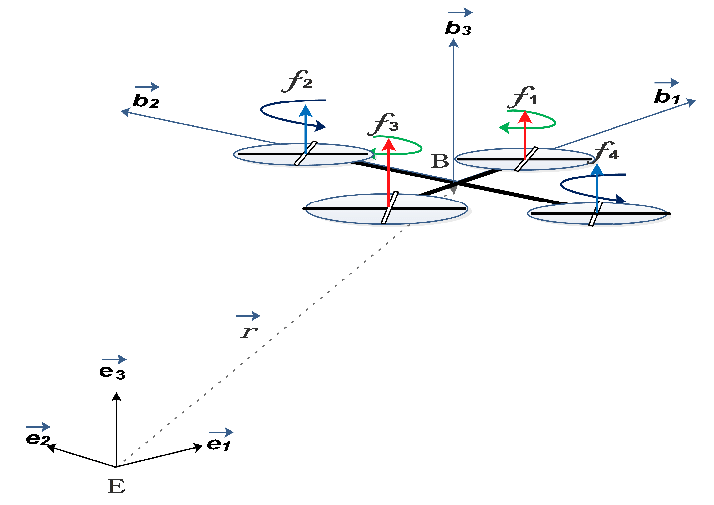
\includegraphics[width=\textwidth]{model.png}
	\caption{Vizualni prikaz letjelice i koordinatnih osi.}
\end{figure}
Napomena: svi parametri modela letjelice nalaze se na github repozitoriju u morus\_description ROS paketu.
\todo[inline]{spomenuti morusa i pokretne mase staviti referencu na github}
\chapter{Geometrijsko upravljanje}

	\section{Uvod}
	
	\paragraph{}Ako se pri upravljanju sustavima njegov konfiguracijski prostor, odnosno njegove varijable stanja, shvaća kao glatki manifold tada se govori o geometrijskom upravljanju sustavima. Kao što je već rečeno, jedna od prednosti pri upravljanju u prostoru manifolda jest koordinatna invarijantnost. Nakon što je odabran i fiksiran početni koordinatni sustav svo daljnje upravljanje je neovisno o trenutnoj konfiguraciji sustava. \\
	Neka je definiran sustav:
	
	\begin{equation}
		\dot{x}=f(x), \, x \in M
	\end{equation}
	Uvodi se pojam vektorskih polja kao skup svih mapa od manifolda M prema TM, odnosno tangencijalnom svežnju (unija svih tangencijalnih prostora $T_xM ,\, \forall x\in M$). \\
	Tada je f jedno vektorsko polje, tj. glatka mapa od manifolda prema tangencijalnom prostoru $T_xM$. Dakle dinamički sustav je vektorsko polje, tj. određen je tokom samo jednog vektorskog polja i ovisi o početnim uvjetima. Pod tokom vektorskog polja misli se na krivulju $x(t)$ kao rješenje sustava. \\
	Kako bi se upravljalo dinamičkim sustavom mora se uzeti u obzir familija vektorskih polja $f(\cdot, u)$ parametrirana sa upravljačkom varijablom $u$. \\
	\begin{equation}
		\dot{x} = f(x(t),\, u(t)), \, x(t)\in M, \, u(t)\in \Ua \subset \mathbb{R}^m
	\end{equation}
	\begin{figure}[h!]
		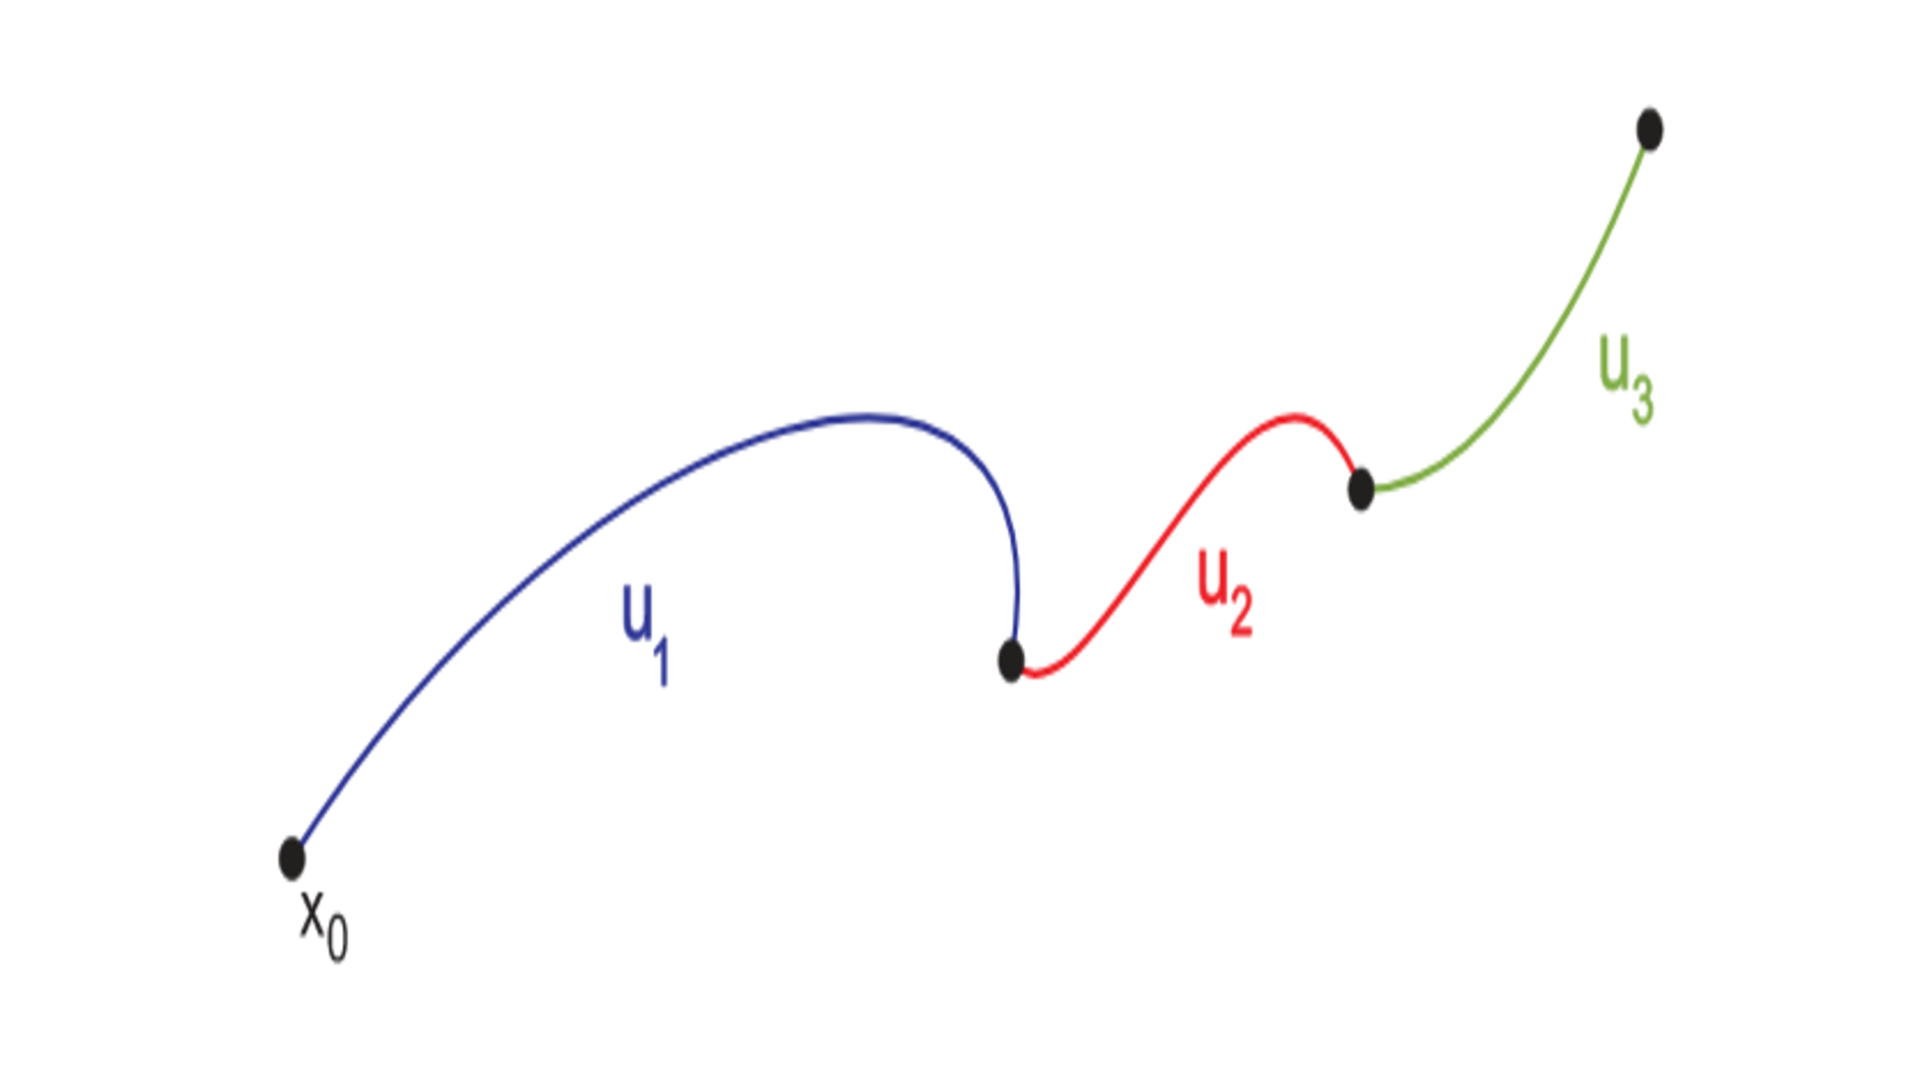
\includegraphics[width=\textwidth, height=5cm]{krivulja.png}
		\caption{Krivulja rješenja sustava uz dodane upravljačke funkcije $u_1(t)$, $u_2(t)$ i $u_3(t)$}
	\end{figure}
	
	\newpage
	\clearpage
	
\section{Geometrijsko upravljanje letjelicom}
	
	\paragraph{}Ukoliko se promatra sustav letjelice tada su varijable stanja razvijene na manifoldu Lijeve grupe SE(3), njihove derivacije leže na vektorskim poljima, odnosno tangencijalnom svežnju koji tada čini Lijevu algebru $se(3)$. Dakle elementi Lijeve grupe predstavljat će konfiguracije, tj. orijentaciju i pomak sustava letjelice dok elementi Lijeve algebre će predstavljati njene kutne, odnosno linearne brzine. \\
	Jedna od prednosti ovakvog načina upravljanja javlja se prilikom prikaza orijentacije sustava pomoću rotacijske matrice koja jasno definira vektore lokalnog koordinatnog sustava. Kod klasičnog upravljanja korištenjem Eulerovih kuteva javljaju se singulariteti. Ako je definiran neki redoslijed rotacija oko osi (npr. $x \rightarrow y \rightarrow z$) te ako je druga po redu rotacija za kut 90 ili 270 tada se dešava tzv. \textit{"Gimbal lock"}. U tom trenutku se gubi 5jedan stupanj slobode, odnosno preostale dvije rotacije se odvijaju oko iste osi.
	
	\begin{figure}[h!]
		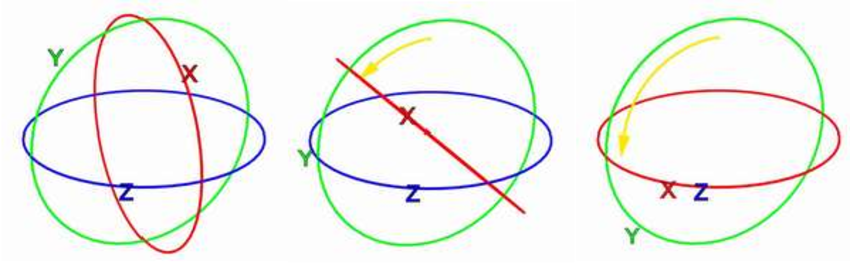
\includegraphics[width=\textwidth]{gimbal_lock.png}
		\caption{Prikaz preklapanja osi prilikom Eulerovih rotacija. Na desnoj slici može se vidjeti kako će rotacije oko x i z osi biti istovjetne.}
	\end{figure}
	
	\noindent Prilikom predstavljanja orijentacije putem kvaterniona ne javlja se problem singulariteta, ali zato se pojavljuje problem dvosmislenosti. Drugim riječima kvaternioni $q$ i $-q$ predstavljaju isti kvaternion, odnosno istu rotaciju u prostoru. Opisani problemi ne pojavljuju se prilikom predstavljanja orijentacije sustava kao element Lijeve grupe SO(3). \\
	Geometrijsko upravljanje letjelicom svodi se na izračunavanje ukupne sile potiska svih rotora te momenata oko osi lokalnog sustava na temelju zadanih vrijednosti pozicije, linearne brzine i akceleracije, odnosno orijentacije, kutne brzine i akceleracije. Sama struktura regulatora je kaskadna, prvo se računa smjer i ukupni iznos sile potiska na temelju pozicijskih referenci te zatim momenti na temelju orijentacijskih referenci. Naposlijetku se dobivene upravljačke vrijednosti sile potiska i momenata preračunavaju u brzine zakreta rotora kako bi se mogle primijeniti na sustav letjelice.

	\newpage
	\clearpage

	\begin{figure}[h!]
		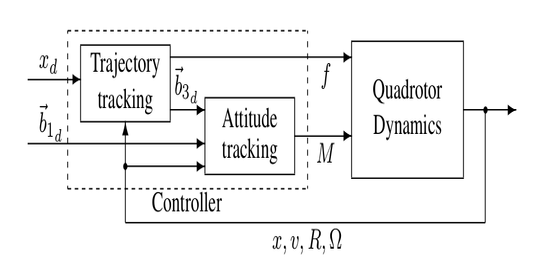
\includegraphics[width=\textwidth, height=5cm]{controller.png}
		\caption{Prikaz kaskadne strukture geometrijskog kontrolera.}
	\end{figure}
	
	U nastavku bit će prikazana sinteza upravljčkog zakona, no najprije će biti potrebno definirati funkcije pogreške. To će biti lako napraviti za praćenje pozicije budući da je se ono odvija unutar translacijske grupe T(3) čiji su elementi dio $\mathbb{R}^3$. Pogreške orijentacije i kutne brzine bit će potrebno pažljivo definirati budući da leže unutar grupe SO(3), odnosno unutar njenog tangencijalnog prostora.
	
\section{Pogreške praćenja reference}

	\paragraph{}Prije nego se započne sinteza geometrijskog regulatora potrebno je definirati funkcije pogrešaka pozicije, orijentacije te linearne i kutne brzine s obzirom na željenu vrijednost (u ostatku teksta sadrži d - \textit{desired} u subskriptu) i trenutnu vrijednost. \\
	Pogreške u poziciji i linearnoj brzini kao translacijski dio SE(3) grupe dane su kao:
	\begin{gather}
		e_x = x - x_d \\
		e_v = v - v_d
	\end{gather}
	
\chapter{Analiza simulacije}
\chapter{Zaključak}
Zaključak.

\bibliography{literatura}
\bibliographystyle{fer}

\begin{sazetak}
Ravijen je nelinearni geometrijski regulator za upravljanje multirotorskom letjelicom s benzinskim motorima. Regulator je implementiran u programskom jeziku C++ u ROS okruženju te ispitan korištenjem simulacijskog okruženja Gazebo na postojećem modelu multirotorske bespilotne letjelice s benzinskim motorima i pokretnim masama.

\kljucnerijeci{geometrijsko upravljanje, multirotorska letjelica, Lijeve grupe, SE(3), ROS, Gazebo}
\end{sazetak}

% TODO: Navedite naslov na engleskom jeziku.
\engtitle{Title}
\begin{abstract}
A nonlinear geometric controller is implemented using C++ programming language within ROS environment. The controller is used on a multirotor unmanned aerial vehicle with internal combustion engines. Results are obtained from Gazebo simulation environment using the existing multirotor UAV model with internal combustion engines and moving masses.

\keywords{geometric control, multirotor UAV, Lie groups, SE(3), ROS, Gazebo}
\end{abstract}

\chapter{literatura}
\end{document}
